\chapter{The Physics of Accretion}

\label{sec:PhysAcc}

\section{The Shakura-Sunyaev Disk Model}

\section{The Eddington Limit}

\subsection{Disk Instabilities}

\label{sec:diskinstab}

L-E xxxxx Using the assumptions present in the thin disk models of \citealp{Shakura_Disk} and \citealp{Novikov_Torque}, \citealp{Lightman_Instability} show that an annulus within a thin, radiatively dominated disk has an effective negative radial diffusion coefficient.  As such, any initially smooth disk under these conditions tends to separate into dense annuli.

\section{GRS 1915+105 and IGR J17091-3624}

xxxxx

\subsection{A History of Models of GRS 1915-like Variability}

\par Over the years, a number of models and physical scenarios have been suggested to explain the complex variability seen in GRS 1915-like systems.  Successful models must also be able to explain why this type of variability is not seen in a wider array of sources.
\par One of the most best-studied classes of GRS 1915-like variability is Class $\rho$, the `heartbeat' class.  This variability class is also present in IGR J17091 (e.g. \citealp{Altamirano_IGR_FH}), and has been the focus of many of the models proposed to explain GRS 1915-like variability.  It has been shown that hard X-ray photons lag soft X-ray photons in this class (e.g. \citealp{Janiuk_Lag,Massaro_Lag}).  Other classes in GRS 1915 which show quasi-periodic flaring behaviour also exhibit this phase lag.
\par Previous authors have established models to explain both the hard photon lag as well as the `heartbeat'-like flaring itself, generally based on the instability in a radiation-dominated disk first reported by \citealp{Lightman_Instability} (see Section \ref{sec:diskinstab}).
\par \citealp{Belloni_Model1} first proposed an empirical model for flaring in GRS 1915.  They suggested that this behaviour is due to a rapid emptying of a portion of the inner accretion disk, followed by a slower refilling of this region over a viscous timescale.  These authors divided data from a given observation into equal-sized 2-Dimensional bins in count rate-colour space.  A spectral model was then fit to each of these bins independently to perform `pseudo'-phase-resolved spectroscopy (compare with the method outlined in Section \ref{sec:phasresspec}).  They showed that the quiescent time between flaring events correlates with the maximum inner disk radius during the flare; i.e., a correlation between the amount of the disk which is emptied and the time needed to refill it.  They go on to suggest that their model is able to explain all flaring-type events seen in GRS 1915.
\par The scenario proposed by \citealp{Belloni_Model1} was mathematically formalised by \citealp{Nayakshin_GRSModel}, who found that it was not consistent with a `slim' accretion disk \citep{Abramowicz_Slim} or with a disk in which viscosity $\alpha$ is constant with respect to radius.  As such, their model consists of a cold accretion disk with a modified viscosity law, a non-thermal electron corona and a transient jet of discrete plasma emissions which are ejected when the bolometric luminosity approaches the Eddington Limit.  Using this model, \citealp{Nayakshin_GRSModel} found that some formulations of $\alpha(r)$ result in the disk oscillating between two quasi-stable branches in viscosity-temperature space, over timescales consistent with those seen in the flaring of GRS 1915; they found that this occurs for accretion rates greater than 26\% of the Eddington limit.  They also found that by varying the functional form of $\alpha(r)$, their model gives rise to a number of lightcurve morphologies which generally match what is seen in data from GRS 1915.  \citealp{Janiuk_RadInstab} built on this model further by including the effect of the transient jet in cooling the disk; an effect not considered in the model by \citealp{Nayakshin_GRSModel}.  In this formulation, \citealp{Janiuk_RadInstab} found that GRS 1915-like variability should occur at luminosities as low as 16\% of Eddington.
\par \citealp{Belloni_GRS_MI} found that variability in GRS 1915 can be described by transitions between three phenomenological states, which differ in luminosity and hardness ratio.  This phenomenological scenario is at odds with the model of \citealp{Nayakshin_GRSModel}, which only results in two quasi-stable states.
\par \citealp{Nobili_Hotspot} tried to account for the hard X-Ray lag by supposing that a significant proportion of the X-Ray variability from the accretion disk comes from a single hotspot.  They suggest that the lag corresponds to a light travel time, after which a portion of this emission is Comptonised by the jet.  In this case, the geometric location of this hotspot determines the magnitude of this lag, and whether it is positive or negative.  This scenario goes some way to explaining why GRS 1915 is special, as it requires the presence of a jet during a soft-like state.
\par \citealp{Tagger_MagneticFlood} propose a magnetic explanation for the ejection of the inner accretion disk required by \citealp{Nayakshin_GRSModel} and \citealp{Janiuk_RadInstab}.  They suggest a limit cycle in which a poloidal magnetic field is advected towards the inner disk during the refilling of this region.  This field is then destroyed in reconnection events, releasing energy which results in the expulsion of matter from the inner disk.  They suggest that the three quasi-stable states proposed by \citealp{Belloni_GRS_MI} can be explained as states in the inner accretion disk with different values of plasma $\beta$.
\par \citealp{Janiuk_Lag} attempt to explain the hard lag in the heartbeats of GRS 1915 more simply, by proposing that it is caused by the non-thermal corona smoothly adjusting to changes in luminosity from the disk.  They base the variability of the disk on the model of \citealp{Nayakshin_GRSModel}, and show that the presence of a non-thermal corona which reacts to this variability naturally reproduces the lag behaviour seen in Class $\rho$ in GRS 1915.
\par \citealp{Merloni_MagDom} also propose a magnetic explanation for the reformulation of $\alpha(r)$ required by the model of \citealp{Nayakshin_GRSModel}.  Assuming that the viscosity in the accretion disk is dominated by turbulence due to magnetorotational instability, they find that allowing for a magnetically dominated corona naturally allows for the forms of $\alpha(r)$ required by \citealp{Nayakshin_GRSModel}.
\par \citealp{Zheng_Model} suggest that, when the effects of a magnetic field are included, the accretion rate threshold for GRS 1915-like variability should be $\sim50$\% of Eddington; significantly higher than the 16\% or 26\% reported by \citealp{Janiuk_RadInstab} or \citealp{Nayakshin_GRSModel}.  They go on to suggest that this sort of variability is only seen in GRS 1915 due to this source having the highest accretion rate of all permanently soft-state sources.  As such, this scenario still relies on a high accretion rate to trigger GRS 1915-like variability.%  However, magnetohydronamic simulations of a radiation dominated inner disk performed by \citealp{Hirose_Stable} suggest that the thermal instabilities required by models of heartbeat should not arise at any value of accretion rate.
\par \citealp{Xue_Spin} derive a mathematical model of the evolution of a slim accretion disk around a Kerr black hole.  They hypothesize that the spin of the black hole, not the accretion rate, may be the driving factor behind GRS 1915-variability.  However, they find that that the morphology of X-ray lightcurves from such a disk only has a weak dependence on the spin of the black hole, ruling this out as a possible explanation.
\par \citealp{Neilsen_GRSModel} performed phase-resolved spectroscopy of the $\rho$ class in GRS 1915.  They find a hard `spike' after each flare, which they associate with the hard lag in this class previously noted by e.g. \citealp{Janiuk_Lag}.  They propose a scenario in which high-velocity winds formed by the ejection of matter from the inner disk interact directly with the corona after a light travel time.  The corona then re-releases this energy as a hard bremsstrahlung pulse, causing the hard count rate spike seen in phase-resolved spectra.  This scenario is outlined in Figure \ref{fig:WindsModel}.  The authors expand this scenario in \citealp{Neilsen_Rho} to suggest that this mechanism can explain all classes in GRS 1915 which display $\rho$-like flaring.  However, this scenario still relies on the model of \citealp{Nayakshin_GRSModel} to generate the instability in the disk, and it implies that hard photons should always lag soft photons in heartbeat-like variability classes.

\pagebreak
\begin{figure}
  \centering
  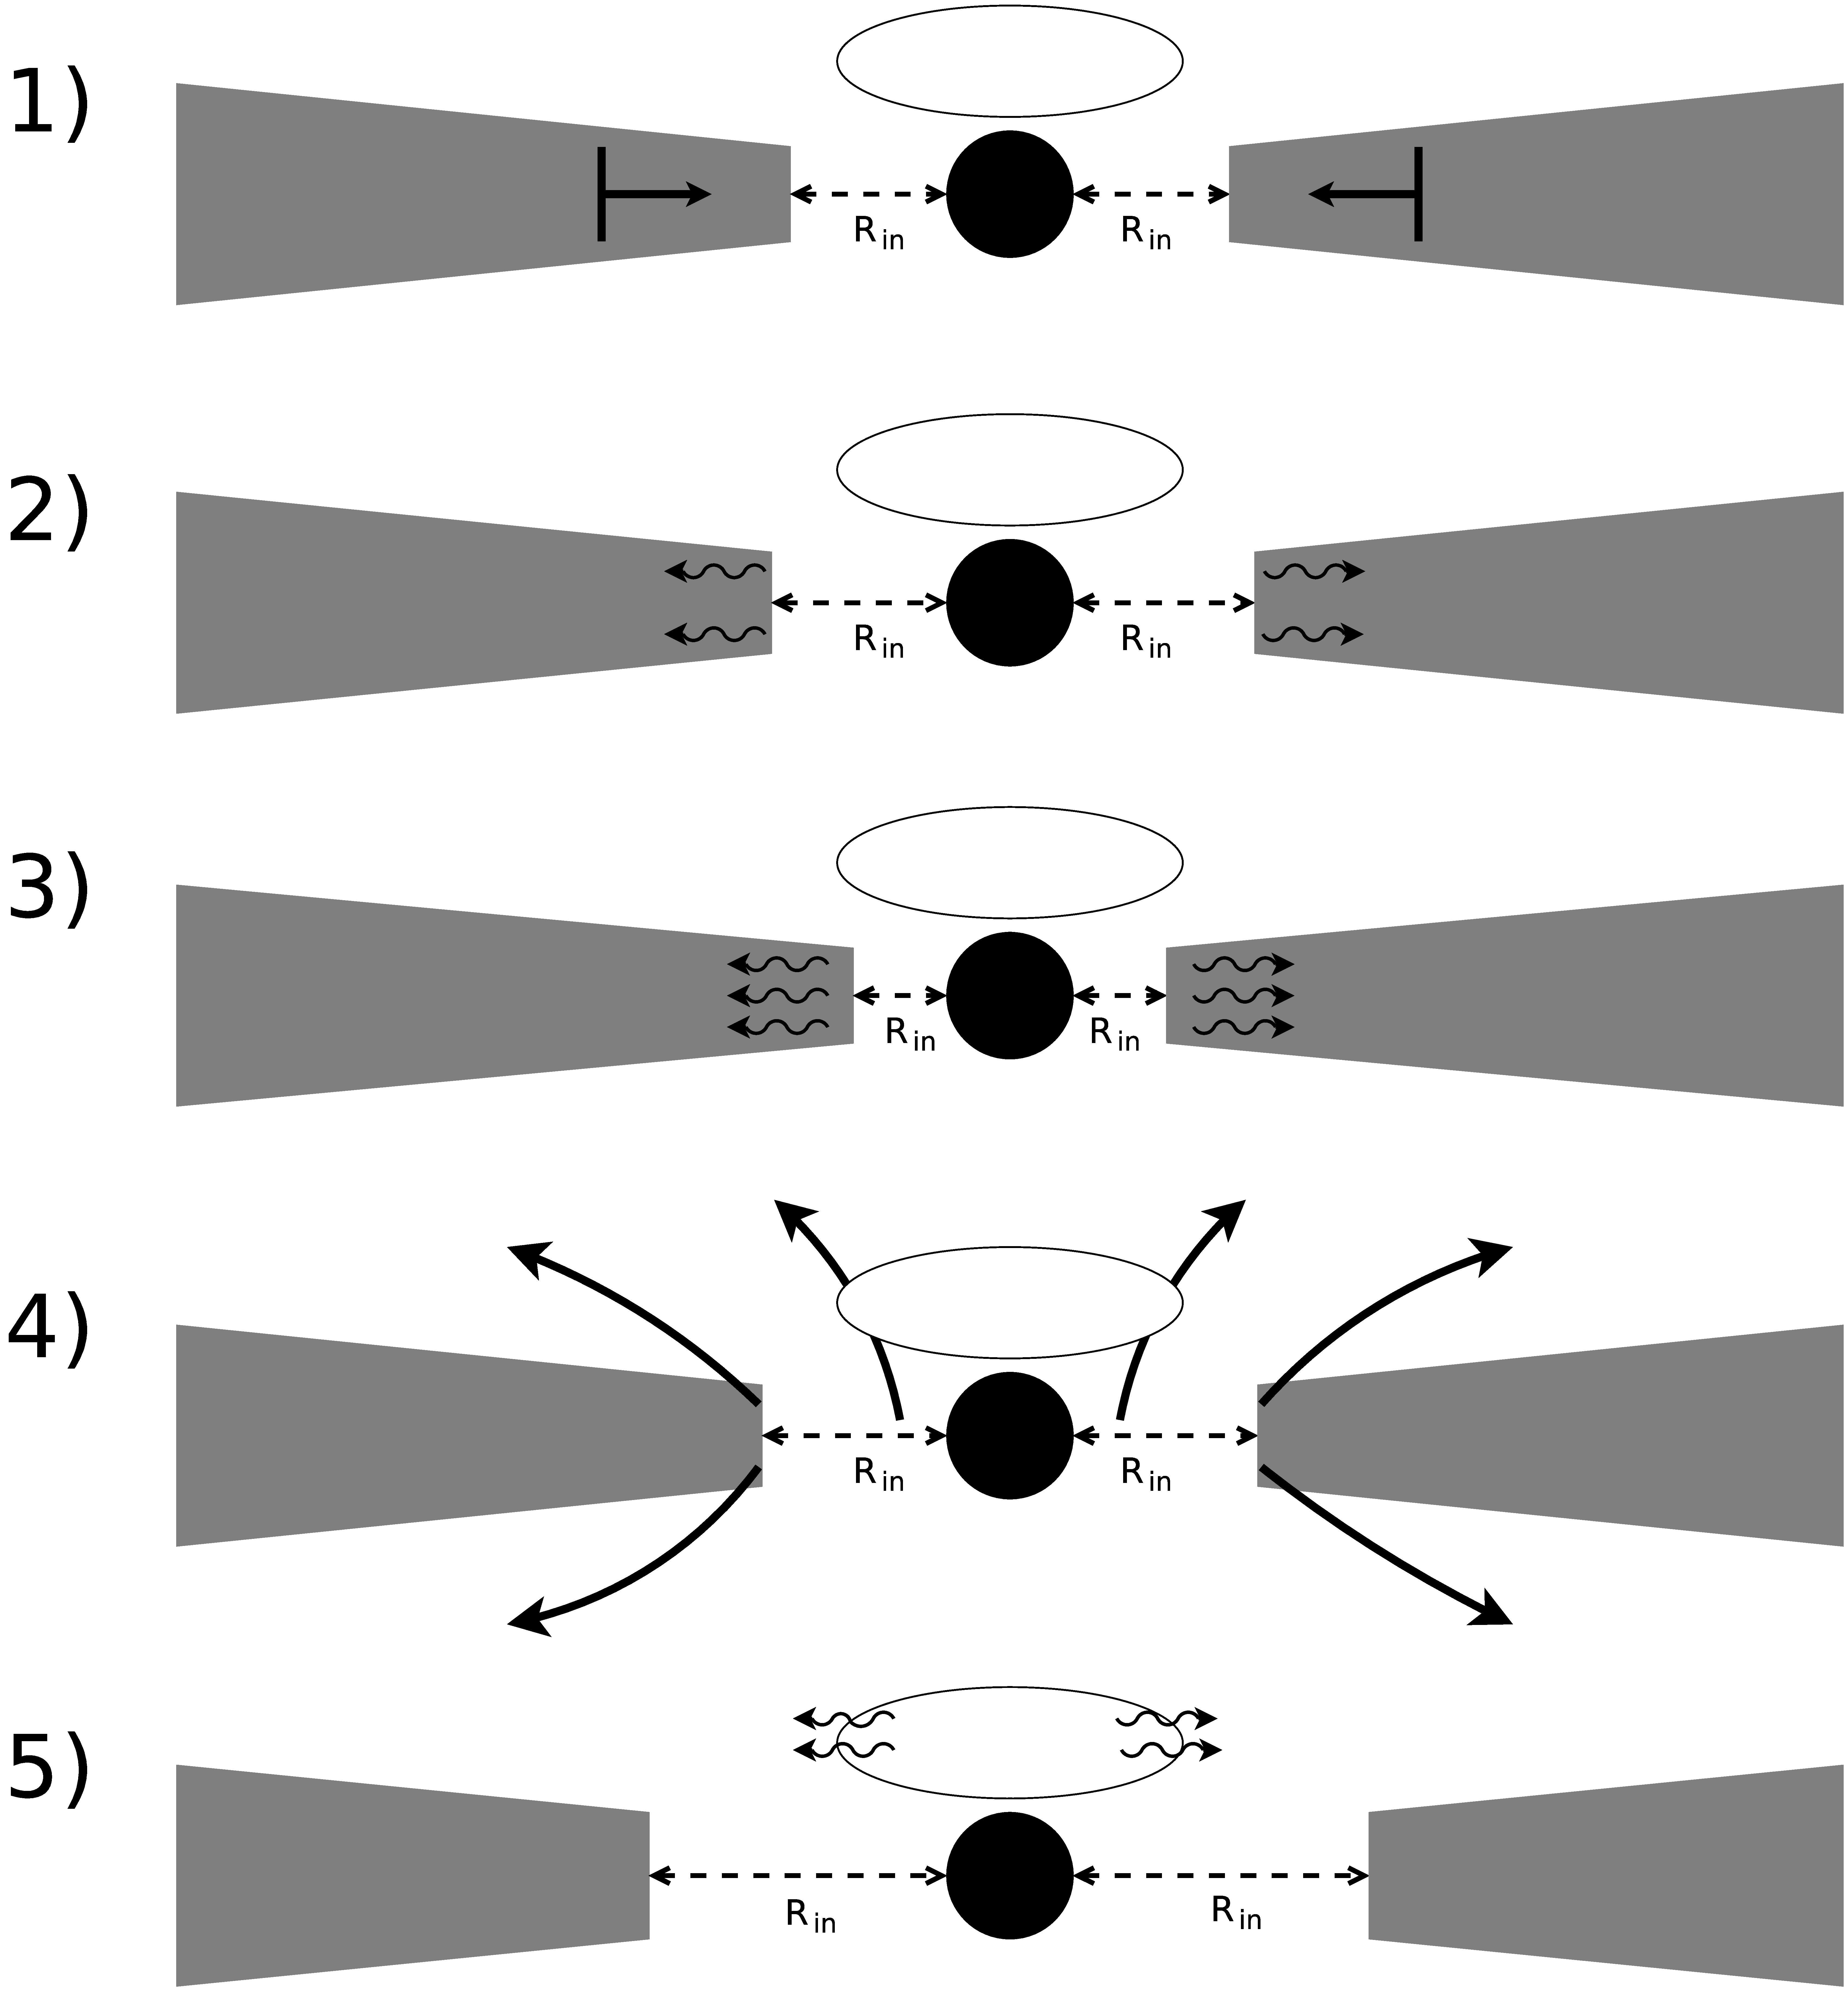
\includegraphics[width=.9\linewidth, trim= 25mm 0mm 0mm 0mm]{images/Wind_Model1.eps}
  \caption{\small A schematic diagram illustrating the the process described by \citet{Neilsen_GRSModel} to describe the $\rho$ variability class in GRS 1915+105.  1) The X-ray emission from the system originates from both the accretion disc truncated at an inner radius $r_{in}$ (grey) and a cloud of non-thermal electrons (white ellipse).  At some time $t$, an overdensity in the accretion disc (formed by the Lightman-Eardley Instability) propagates inwards towards $r_{in}$.  2) As the inner disc heats up, $r_{in}$ begins to slowly increase due to an increase in photon pressure.  This destabilises the disc.  3) At some critical density, the disc becomes too unstable and collapses inwards, greatly decreasing $r_{in}$ and raising the inner disc temperature.  4) The sudden increase in emission exceeds the local Eddington limit at $r_{in}$, ejecting matter from the inner accretion disc in the form of extreme winds.  5) Having been excited by matter in the winds passing through it, the non-thermal electron cloud emits a hard Brehmsstrahlung `pulse'.}
  \label{fig:WindsModel}
\end{figure}
\pagebreak

\par In their fitting, \citealp{Neilsen_GRSModel} consider three spectral models:
\begin{enumerate}
\item An absorbed disk black body with a high energy cutoff, of which some fraction has been Compton upscattered
\item An absorbed disk black body with a high energy cutoff, plus a Compton component with a seed photon spectrum tied to the emission from the disk
\item An absorbed disk black body plus a Compton component with a seed photon spectrum tied to the emission from the disk and a bremsstrahlung component
\end{enumerate}
They find that the first of these models (Model 1) is the best fit to the data.
\par \citealp{Mineo_PhasRes} also performed psuedo-phase-resolved spectroscopy of the $\rho$ class in GRS 1915, using a number of different spectral models to \citealp{Neilsen_GRSModel} but a significantly lower phase resolution.  In this work, the authors consider six models:
\begin{enumerate}
\item A multi-temperature disk black body plus a corona containing both thermal and non-thermal electrons (as forumlated by \citealp{Poutanen_Hybrid})
\item A multi-temperature disk black body plus a multi-temperature disk black body plus a power law
\item A multi-temperature disk black body plus an independent Compton component
\item A multi-temperature disk black body plus a power law plus reflection from the outer disk
\item A model of Comptonization due to the bulk-motion of matter in the disk
\item A multi-temperature disk black body plus a power law plus a standard black body
\end{enumerate}
With the exception of Models \textit{i} and \textit{vi}, the authors find that none of these models are able to satisfactorily fit the data in each of their phase bins independently.  As there is no reasonable physical explanation behind Model \textit{vi}, the authors only consider Model \textit{i}.  Their results suggest a large reduction of the corona luminosity during each heartbeat flare, which they interpret as the corona condensing onto the disk.  They also find that their results are consistent with GRS 1915 having a slim disk, but inconsistent with the hard lag being caused by photon upscattering in the corona.
\par \citealp{Massa_MoveLag} found that the magnitude of the lag between hard and soft photons in the $\rho$-class of GRS 1915 is not constant.  They found that the lag varies between $\sim3$--$10$\,s, and correlates strongly with count rate.  The magnitude of the lag, therefore, is too large to be simply due to a light travel time to the corona from the disk.  The authors suggest that their results are instead consistent the thermal adjustment of the inner disk itself as part of the instability limit cycle invoked to explain the flares.
\par \citealp{Massaro_Numerical} constructed a set of differential equations to mathematically explain the behaviour of the oscillator underlying $\rho$-like flaring in GRS 1915.  They find that a change between variability classes likely corresponds to a a change in global accretion rate, but that the accretion rate within the $\rho$ class is constant.  This model reproduces the count rate-lag correlation reported by \citealp{Massa_MoveLag}, as well as a previously reported correlation between flare recurrence time and count rate \citep{Massaro_Lag}.
\par \citealp{Mir_LagModel} instead propose a model of variability in the outer disk propagating inwards to the hotter inner disk.  They propose a model that explains both the hard lag of the fundamental frequency associated with the heartbeat flares, but also the hard lag of the first harmonic.  In contrast to the findings of \citealp{Massaro_Numerical}, their scenario requires a sinusoidal variation in the global accretion rate as a function of time.
\par More recently, \citealp{Zoghbi_Bulge} found that the reflection spectrum from GRS 1915 does not match what would be expected from the inner disk behaviour assumed by e.g. \citealp{Nayakshin_GRSModel}.  They again perform phase-resolved spectroscopy and fit a number of complex spectral models, finding that their data is best-described by the emergence of a bulge in the inner disk which propagates outwards during each flare.

\section{Type II Burst Sources}

xxxxx